\documentclass[fleqn, 12pt]{article}
% Packages
\usepackage[0.9, font.kp, swapVarGreek]{sigilz}
\usepackage{hyperref}
\usepackage{url}

\usepackage{listings}
\usepackage{color}

\definecolor{dkgreen}{rgb}{0,0.6,0}
\definecolor{gray}{rgb}{0.5,0.5,0.5}
\definecolor{mauve}{rgb}{0.58,0,0.82}
\lstset{frame=tb,
  aboveskip=3mm,
  belowskip=3mm,
  showstringspaces=false,
  columns=flexible,
  basicstyle={\small\ttfamily},
  keywordstyle=\color{blue},
  commentstyle=\color{dkgreen},
  stringstyle=\color{mauve},
  breaklines=true,
  breakatwhitespace=true,
  tabsize=3
}

% Header
\setlength{\headheight}{15pt}
\pagestyle{fancy}
\lhead{Adam B Jones and Fei Yuan}
\chead{PHY982}
\marginparsep=2cm

% Environments
\definecolor{correctioncolor}{rgb}{.7, .2, 0}
\provideenvironment{correction}{\begingroup\color{correctioncolor}}{\endgroup}
\provideenvironment{valigntop}%
{\begin{minipage}[t]{\textwidth}\vspace{0pt}}%
{\vspace{0pt}\end{minipage}}

% Commands
\providecommand{\Dom}{\operatorname{Dom}}
\providecommand{\Roots}{\operatorname{Roots}}
\providecommand{\pvint}{\fint}
\providecommand{\integral}{\mathop{\textstyle\int}}
\providecommand{\ointegral}{\mathop{\textstyle\oint}}
\def\oint{\ointctrclockwise}

% note: \textcolor for fg; \colorbox for bg
\definecolor{rescolor}{rgb}{.8, .9, 1}
\newcommand{\resmath}[1]{\colorbox{rescolor}{\ensuremath{\displaystyle
      #1}}}

\rhead{HW3}
\begin{document}

\begin{enumerate}

\item
  \begin{figure}
    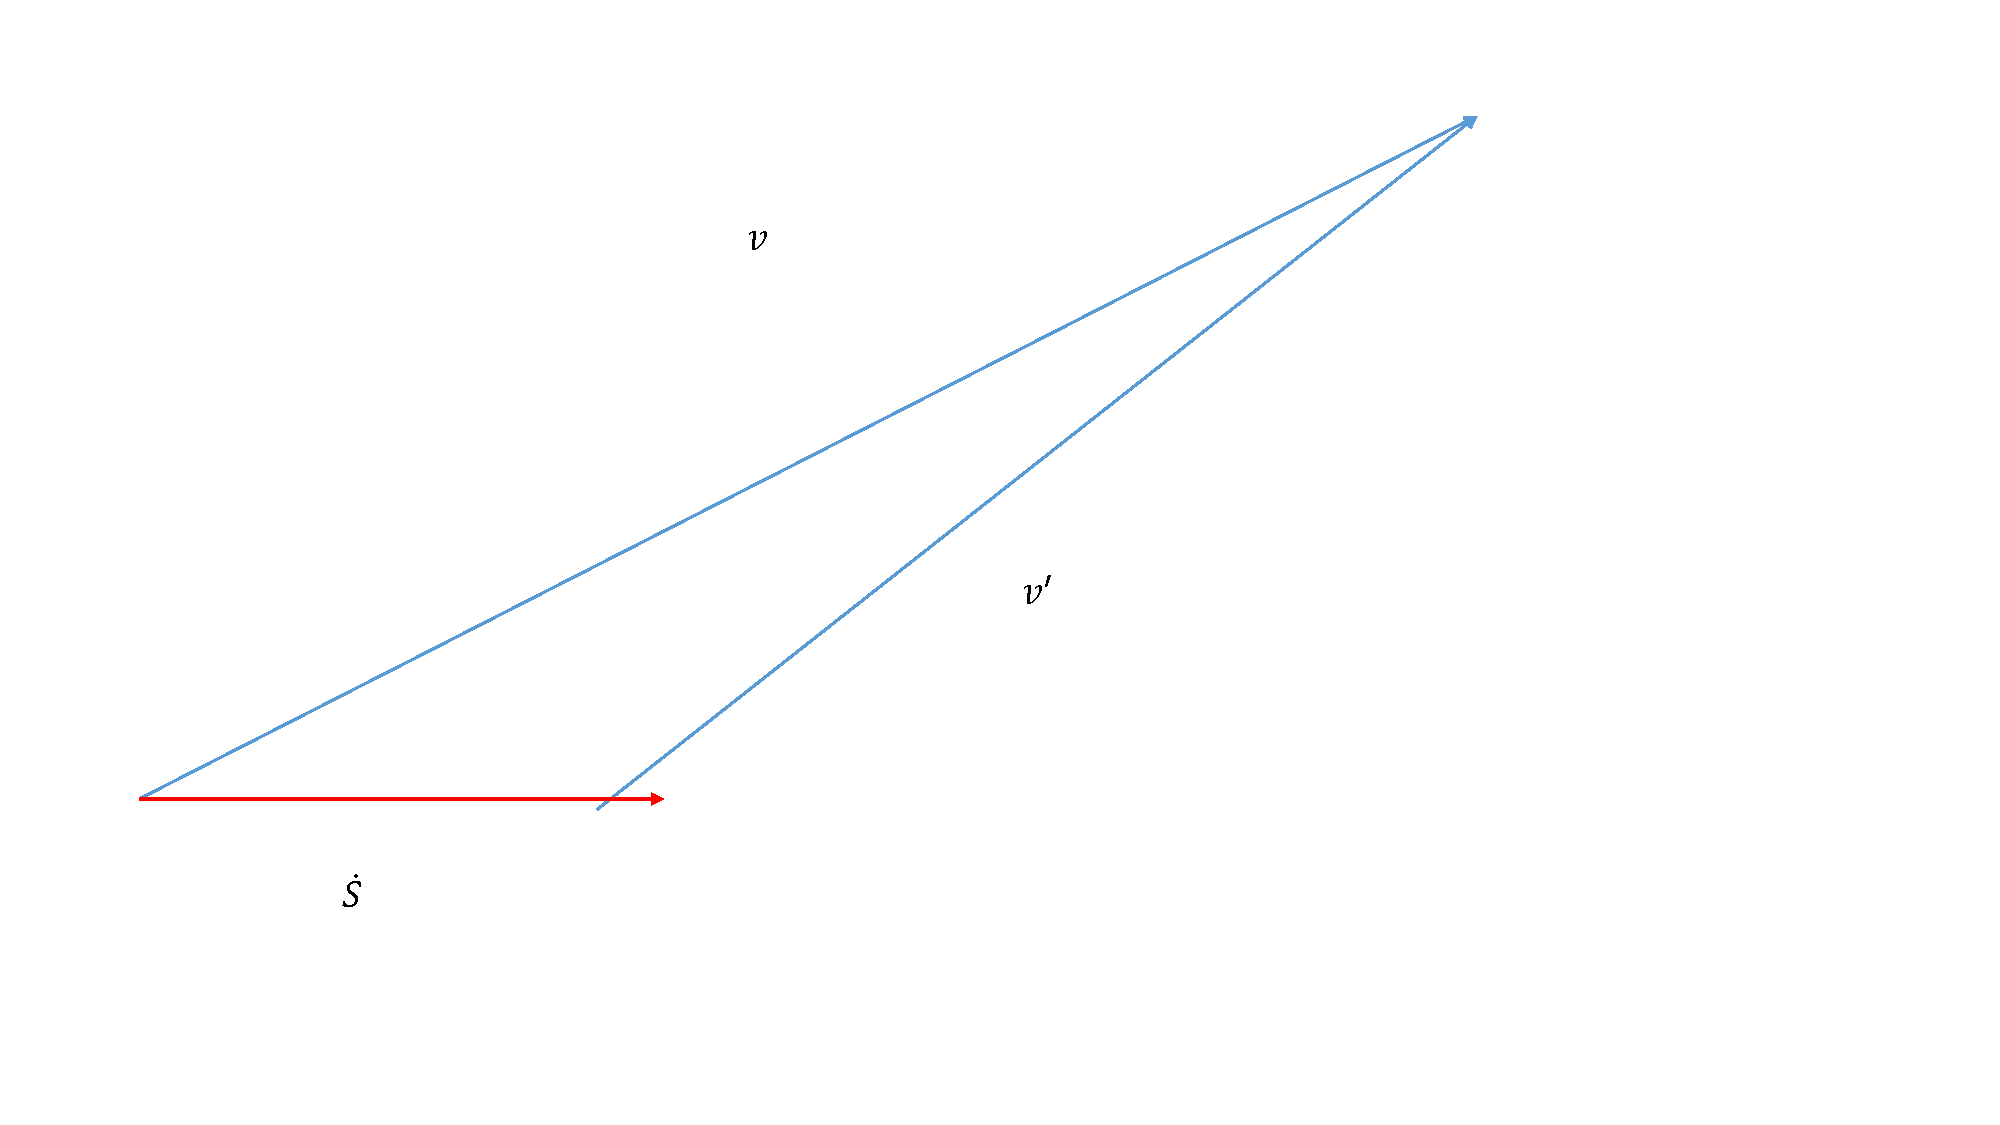
\includegraphics[width=\textwidth]{hw3-comlab.pdf}
    \caption{The relation between CM and Lab frames.}
    \label{fig:comlab}
  \end{figure}

  The relationship between the center-of-mass and lab velocities is given by
  the following equations and can be seen in Figure \ref{fig:comlab}:
  \begin{align*}
    v_{\text c}' \sin \theta &= v_{\text c} \sin \theta_{\text{lab}} \\
    \dot S + v_{\text c}' \cos\theta &= v_{\text c} \cos \theta_{\text{lab}} \\
    \phi &= \phi_{\text{lab}} \\
    \bm v_{\text c} &= \bm v_{\text c}'+ \dot{\bm S}
  \end{align*}
  Define the parameter $\rho \equiv \dot S / v_{\text c}'$.  The relationship between
  the lab and center-of-mass scattering angles can be expressed as:
  \begin{align*}
  \tan\theta_{\text{lab}}=\frac{\sin\theta}{\rho+\cos\theta}
  \end{align*}
  We also know that conservation of flux requires the scattering cross section
  in an infinitesimal solid angle to be conserved by the change in reference
  frame.  This leads to the following expression:
  \begin{align*}
    &\frac{\D \sigma_{\text{lab}}}{\D \Omega} (\theta_{\text{lab}}, \phi_{\text{lab}})
      \D \phi_{\text{lab}} \sin \theta_{\text{lab}} \D \theta_{\text{lab}}
      = \frac{\D \sigma}{\D \Omega} (\theta, \phi)
      \D \phi \sin \theta \D \theta \\
    &\Rightarrow
      \frac{\D \sigma_{\text{lab}}}{\D \Omega}
      (\theta_{\text{lab}}, \phi_{\text{lab}})
      = \frac{\D \sigma}{\D \Omega} (\theta, \phi)
      \frac{\D \phi}{\D \phi_{\text{lab}}}
      \frac{\sin \theta}{\sin \theta_{\text{lab}}}
      \frac{\D \theta}{\D \theta_{\text{lab}}}
  \end{align*}
  Clearly, $\D \phi / \D\phi_{\text{lab}} = 1$ and
  \begin{align*}
    \frac{\sin \theta}{\sin \theta_{\text{lab}}}
    = \frac{v_{\text c}}{v_{\text c}'}
    = \frac{\sqrt{\bm v_{\text c} \cdot \bm v_{\text c}}}{v'}
    = \frac{\sqrt{v_{\text c}^2 + 2 v_{\text c} \dot S \cos \theta + \dot S^2}}{v'}
    = \sqrt{1 + 2 \rho \cos \theta + \rho^2}
  \end{align*}
  To find the the derivative of $\theta$:
  \begin{align*}
    &\frac{\D}{\D \theta_{\text{lab}}} \tan \theta_{\text{lab}} =
      \frac{\D}{\D \theta_{\text{lab}}} \frac{\sin \theta}{\rho + \cos \theta} \\
    &\sec^2 \theta_{\text{lab}}
      = \frac{1 + \rho \cos \theta}{(\rho + \cos\theta)^2}
      \frac{\D \theta}{\D \theta_{\text{lab}}} \\
    &\Rightarrow \frac{\D \theta}{\D \theta_{\text{lab}}} =
      \cos^2 \theta_{\text{lab}}
      \frac{1 + \rho \cos \theta}{\left(\rho + \cos \theta\right)^2}
  \end{align*}
  But
  \begin{align*}
    &\cos^2 \theta_{\text{lab}}
    = \left(\frac{\dot S + v_{\text c}' \cos \theta}{v_{\text c}}\right)^2
    = \left(\frac{v_{\text c}'}{v_{\text c}}\right)^2 (\rho + \cos \theta)^2 \\
    &\Rightarrow \frac{\D \theta}{\D \theta_{\text{lab}}}
    =\left(\frac{v_{\text c}'}{v_{\text c}}\right)^2 \left(1 + \rho \cos \theta\right)
  \end{align*}
  So we have:
  \begin{align*}
    \frac{\D \sigma_{\text{lab}}}{\D \Omega} (\theta, \phi)
    &= \left(\frac{v_{\text c}'}{v_{\text c}}\right)^3
      \frac{1}{1 + \rho \cos \theta}
      \frac{\D \sigma}{\D \Omega} (\theta, \phi) \\
    &= \frac{\left(1 + 2 \rho \cos \theta + \rho^2 \right)^{3/2}
      }{1 + \rho \cos \theta}
      \frac{\D \sigma}{\D \Omega} (\theta, \phi)
  \end{align*}

\item Assume we have a short-ranged, spherically symmetric potential $V(r)$.
  The incident beam is a plane wave of momentum of $k$ originating from the
  negative z-axis:
  \begin{align*}
    \psi_{\text i}(\bm r) = \E^{\I k z}
  \end{align*}
  The scattered wave has the asymptotic form
  \begin{align*}
    \psi_{\text f}(\bm r) = f(\theta) \frac{\E^{\I k r}}{r}
  \end{align*}
  where we have omitted the azimuth $\phi$ due to symmetry.

  The Schr\"odinger equation of this problem is:
  \begin{align*}
    \left(-\frac{\hbar^2}{2 m} \nabla^2 + V(r)\right) \psi(\bm r)
    = E \psi(\bm r)
  \end{align*}
  In spherical coordinates, the Laplacian is given by:
  \begin{align*}
  -\nabla^2 = \frac{1}{r^2} (\hat \ell^2 - \frac{\D}{\D r} r^2 \frac{\D}{\D r})
  \end{align*}
  where $\hat{\bm \ell}$ is the orbital angular momentum operator, whose
  eigenvalues are of the form $\ell (\ell + 1)$.  Due to azimuthal symmetry,
  the only possible angular eigenstates are the ones with $m = 0$, which are
  simply the Legendre polynomials composed with cosine: $P_\ell(\cos \theta)$.

  Hence, we shall expand the incoming wave as a sum of Legendre polynomials:
  \begin{align*}
    \E^{\I k z} =
    \sum_{\ell = 0}^\infty a_\ell P_\ell(\cos \theta)
  \end{align*}
  To do this, we use the orthogonality relations
  \begin{align}
     \int_0^\PI P_\ell(\cos \theta) P_{\ell'}(\cos \theta) \sin \theta \D \theta
    = \frac{2}{2 \ell + 1} \Kroneckerdelta_{\ell \ell'}
    \label{eq:legendre-orthogonality}
  \end{align}
  to obtain the coefficients:
  \begin{align*}
     \frac{2}{2 \ell + 1} a_\ell
    = \int_0^\PI P_\ell(\cos \theta) \E^{\I k r \cos \theta} \sin \theta \D \theta
  \end{align*}
  According to NIST 10.54.3 (\url{http://dlmf.nist.gov/10.54#E2}), this
  integral is proportional to the spherical Bessel function:
  \begin{align*}
    \dots = \frac{2}{(-\I)^\ell} j_\ell(k r)
  \end{align*}
  Thus,
  \begin{align*}
    \E^{\I k z} =
    \sum_{\ell = 0}^\infty (2 \ell + 1) \I^\ell j_\ell(k r) P_\ell(\cos \theta)
  \end{align*}
  The spherical Bessel functions $j_\ell$ (regular) and $y_\ell$ (irregular)
  are related to the Riccati--Hankel functions $\zeta_\ell$ (incoming) and
  $\xi_\ell$ (outgoing) by:
  \begin{align*}
    &\zeta_\ell(s) = s (j_\ell(s) - \I y_\ell(s)) \\
    &\xi_\ell(s) = s (j_\ell(s) + \I y_\ell(s))
  \end{align*}
  Therefore, the plane waves may also be written as:
  \begin{align*}
    \E^{\I k z} =
    \sum_{\ell = 0}^\infty (2 \ell + 1) \I^\ell
    \frac{1}{2 k r} (\zeta_\ell(k r) + \xi_\ell(k r)) P_\ell(\cos \theta)
  \end{align*}
  In this form, the partial wave S-matrix element $S_\ell$ is defined as the
  coefficient of the outgoing wave in the asymptotic wave function:
  \begin{align*}
    \psi(\bm r) \sim \sum_{\ell = 0}^\infty (2 \ell + 1) \I^\ell
    \frac{1}{2 k r} (\zeta_\ell(k r) + S_\ell \xi_\ell(k r)) P_\ell(\cos \theta)
  \end{align*}
  The incoming wave must have the same coefficient as that of the plane wave
  due to the boundary conditions.

  The scattered wave $\psi_{\text f}$ is the difference between the full wave
  function $\psi$ and the incident plane wave $\psi_{\text i}$, hence its
  asymptotic form is also their respective difference:
  \begin{align*}
    \psi_{\text f}(\bm r) \sim \sum_{\ell = 0}^\infty (2 \ell + 1) \I^\ell
    \frac{1}{2 k r} (S_\ell - 1) \xi_\ell(k r) P_\ell(\cos \theta)
  \end{align*}
  We can factor out the spherical wave
  \begin{align*}
    \psi_{\text f}(\bm r) \sim \frac{\E^{\I k r}}{r}
    \sum_{\ell = 0}^\infty (2 \ell + 1) \I^\ell
    \frac{1}{2 k} (S_\ell - 1) \frac{\xi_\ell(k r)}{\E^{\I k r}} P_\ell(\cos \theta)
  \end{align*}
  and use the asymptotic behavior of the Riccati--Hankel functions
  \begin{align*}
    \xi_\ell(s) \sim \I^{-(\ell + 1)} \E^{\I s}
  \end{align*}
  to simplify the result for large $r$:
  \begin{align*}
    \psi_{\text f}(\bm r)
    &\sim \frac{\E^{\I k r}}{r}
    \sum_{\ell = 0}^\infty (2 \ell + 1) \I^\ell
    \frac{1}{2 k} (S_\ell - 1) \I^{-(\ell + 1)} P_\ell(\cos \theta) \\
    &=\frac{\E^{\I k r}}{r}
    \frac{1}{2 \I k} \sum_{\ell = 0}^\infty (2 \ell + 1)
    P_\ell(\cos \theta) (S_\ell - 1)
  \end{align*}
  From this, we may read off the scattering amplitude $f$:
  \begin{align*}
    f(\theta) =
    \frac{1}{2 \I k} \sum_{\ell = 0}^\infty (2 \ell + 1)
    P_\ell(\cos \theta) (S_\ell - 1)
  \end{align*}

\item Starting with the relationship between cross section and scattering
  length we can use the result of the previous problem.
  \begin{align*}
    \frac{\D \sigma_{\text{el}}}{\D \Omega} (\theta)
    &= |f(\theta)|^2 \\
    &= \left|\frac{1}{2 \I k}\right|^2
      \left|\sum_{\ell = 0}^\infty (2 \ell + 1)
      P_\ell (\cos \theta) (S_\ell - 1)\right|^2 \\
    &= \frac{1}{4 k^2} \sum_{\ell, \ell' = 0}^\infty
      (2 \ell + 1) P_\ell (\cos \theta) (S_\ell - 1)
      (2 \ell' + 1) P_\ell^* (\cos \theta) (S_{\ell'}^* - 1)
  \end{align*}
  Using the orthogonality of the Legendre polynomials
  \eqref{legendre-orthogonality},
  \begin{align*}
    &\eqbegin 2 \PI \int_0^\PI \frac{\D \sigma_{\text{el}}}{\D \Omega} (\theta)
      \sin \theta \D \theta \\
    &= \frac{\PI}{2 k^2}
      \sum_{\ell, \ell' = 0}^\infty
      (2 \ell + 1) (2 \ell' + 1)
      (S_\ell - 1) (S_{\ell'}^* - 1)
      \int_0^\PI P_\ell(\cos \theta) P_\ell^*(\cos \theta) \D \theta \\
    &= \frac{\PI}{2 k^2}
      \sum_{\ell, \ell' = 0}^\infty
      (2 \ell + 1) (2 \ell' + 1) (S_\ell - 1) (S_{\ell'}^* - 1)
      \frac{2 \Kroneckerdelta_{\ell \ell'}}{2 \ell + 1}
  \end{align*}
  Evaluating the sum over $\ell'$ yields:
  \begin{align*}
    \frac{\D \sigma_{\text{el}}}{\D \Omega}(\theta)
    &= \frac{\PI}{k^2} \sum_{\ell = 0}^\infty (2 \ell + 1) (|S_\ell|^2 - (S_\ell + S_\ell^*) + 1)
    = \frac{2 \PI}{k^2} \sum_{\ell = 0}^\infty (2 \ell + 1) (1 - \Re S_{\ell})
  \end{align*}
  Here we have used the fact that $|S_\ell|^2 = 1$ in elastic scattering.  We
  can write $S_\ell = \E^{\I \phi} \Rightarrow \log S_{\ell} = \I \phi$.  Let
  $\delta_{\ell} = \frac{\log S_{\ell}}{2 \I} = \frac{\phi}{2}$ be the phase
  shift. This implies
  \begin{align*}
    \Re S_{\ell} = \cos \phi = \cos^2 \frac{\phi}{2} - \sin^2 \frac{\phi}{2}
  \end{align*}
  Therefore we have
  \begin{align*}
    \sigma_{\text{el}}
    &= \frac{2 \PI}{k^2} \sum_{\ell = 0}^\infty (2 \ell + 1)
      (1 - (\cos^2 \delta_\ell - \sin^2 \delta_\ell)) \\
    &= \frac{4 \PI}{k^2} \sum_{\ell = 0}^\infty (2 \ell + 1) \sin^2 \delta_\ell
\end{align*}

\item Assuming a phase shift around a resonance with the usual shape:
  \begin{align*}
    \delta(E) = \delta_{\text{bg}}(E) +
    \operatorname{atan2}\left(\frac{\Gamma}{2}, E_{\text r} - E\right)
  \end{align*}
  The S-matrix element can be recovered by exponentiation:
  \begin{align*}
    S(E)
    &= \left(\E^{\I \delta(E)}\right)^2 \\
    &= \left(\E^{\I \delta_{\text{bg}}(E)}
      \E^{\I \operatorname{atan2}(\Gamma / 2, E_{\text r} - E)}\right)^2
  \end{align*}
  The arguments of $\operatorname{atan2}$ may be interpreted as the phase of a
  complex number with unit magnitude:
  \begin{align*}
    \frac{\I \Gamma / 2 + E_{\text r} - E}{
    |\I \Gamma / 2 + E_{\text r} - E|}
  \end{align*}
  Allowing the exponentiation to cancel the effect of $\operatorname{atan2}$:
  \begin{align*}
    S(E)
    &= \left(\E^{\I \delta(E)}\right)^2 \\
    &= \left(\E^{\I \delta_{\text{bg}}(E)}
      \frac{\I \Gamma / 2 + E_{\text r} - E}{
      |\I \Gamma / 2 + E_{\text r} - E|}\right)^2 \\
    &= \E^{2 \I \delta_{\text{bg}}(E)}
      \frac{(\I \Gamma / 2 + E_{\text r} - E)^2}{
      |\I \Gamma / 2 + E_{\text r} - E|^2} \\
    &= \E^{2 \I \delta_{\text{bg}}(E)}
      \frac{\I \Gamma / 2 + E_{\text r} - E}{
      -\I \Gamma / 2 + E_{\text r} - E} \\
    &= \E^{2 \I \delta_{\text{bg}}(E)}
      \frac{E - E_{\text r} - \I \Gamma / 2}{
      E - E_{\text r} + \I \Gamma / 2}
  \end{align*}
  It is evident from this equation that the S-matrix element is singular when
  $E = E_{\text r} + \I \Gamma / 2$.  In particular, it is a simple pole that,
  when expanded to first order, has the general form above.

  In the complex energy plane, there exists an eigenstate of the Schr\"odinger
  equation with a complex energy of $E_{\text r} + \I \Gamma / 2$.  One can
  infer that it is resonance state because it has a finite lifetime:
  \begin{align*}
    \Psi(\bm r; t) \propto \E^{\I (E_{\text r} + \I \Gamma / 2) t / \hbar}
    = \E^{\I E_{\text r} t / \hbar} \E^{-\Gamma t / (2 \hbar)}
  \end{align*}

\item Starting from Fermi's golden rule we have:
  \begin{align*}
    \D J_{f i} = |M_{f i}|^2 2 \PI \delta(E_f - E_i) \D N_{f}
  \end{align*}
  Our initial and final states consist of free particles:
  \begin{align*}
    &\ket{\Psi_n} = \frac{1}{\sqrt V} \E^{\I \bm p_n \cdot \bm r} \\
    &\Rightarrow M_{f i}
      = \brakket{\Psi_f}{U(\bm r)}{\Psi_i}
      = \frac{1}{V} \int_{\Real^3}
      \E^{\I \bm p_f \cdot \bm r} U(\bm r) \E^{\I \bm p_i \cdot \bm r} \D \bm r
  \end{align*}
  Where $V$ is an arbitrary normalization factor. Since we are interested in
  the Coulomb potential of a nucleus with atomic number $Z$ we have
  $U(\bm r) = Z_1 Z_2 \alpha / r$ thus:
  \begin{align*}
    M_{fi} = \frac{1}{V} \int \E^{\I \bm q \cdot \bm r} \frac{Z_1 Z_2 \alpha}{r} \D \bm r
    = \frac{Z_1 Z_2 \alpha}{V} \frac{4 \PI}{q^2}
  \end{align*}
  where we have used the definition of the momentum transfer
  $\bm q = \bm p_f - \bm p_i$ and the 3D Fourier trasnsform of the Coulomb
  potential $\mathcal F_{\bm r} (1 / r) = 4 \PI / k^2$.

  We can use the canonical relationship between particle current and cross
  section: $\D J = j N \D \sigma$ where $j$ is the magnitude of the
  probability current given by
  \begin{align*}
    \bm j = \frac{\hbar}{2 \I m} (\Psi^* \nabla \Psi - \Psi \nabla \Psi^*)
    = \frac{\hbar \bm p}{m V} = \frac{\hbar \bm v}{V}
  \end{align*}
  So the cross section is
  \begin{align*}
    \D \sigma = \frac{\D J}{j_i N}
    = \frac{|M_{f i}|^2 V}{4 \PI^2 v_i} \delta(E_f - E_i) \D \bm p_f
  \end{align*}
  Using $\D \bm p_f = p_f^2 \D p_f \D \Omega$ and integrating our equation to
  enforce energy conservation:
  \begin{align*}
    \frac{\D \sigma}{\D \Omega}
    &= \frac{|M_{f i}|^2 V}{4 \PI^2 v_i}
      \int \D p_f p_f^2 \delta(E_f - E_i) \\
    &= \frac{|M_{f i}|^2 V}{4 \PI^2 v_i}
      \int \frac{\D p_f}{\D E_f} \D E_f p_f^2 \delta(E_f-E_i) \\
    &= \frac{|M_{f i}|^2 V p_f^2}{4 \PI^2 v_i v_f} \\
    &= \frac{4 (Z_1 Z_2)^2 \alpha^2 p_f^2}{q^4 v_i v_f}
  \end{align*}
  Since our collision is elastic we have $p_f = p_i = p$ so
  $q^2 = (\bm p_f - \bm p_i)^2 = 4 p^2 \sin^2(\theta / 2)$.  Substituting:
  \begin{align*}
    \frac{\D \sigma}{\D \Omega}
    = \frac{4 (Z_1 Z_2)^2 \alpha^2 p^2}{16 p^4 \sin^4 \frac{\theta}{2} v_i v_f}
    = \frac{(Z_1 Z_2)^2 \alpha^2}{4 \hbar^2 k^2 \sin^4 \frac{\theta}{2} v^2}
    = \frac{(Z_1 Z_2)^2 \alpha^2 \mu}{4 \hbar^2 k^2 \sin^4 \frac{\theta}{2} 2 E}
    = \frac{\eta^2}{4 k^2 \sin^4 \frac{\theta}{2}}
  \end{align*}
  where the Sommerfeld parameter $\eta$ is given by:
  \begin{align*}
    \eta \equiv \frac{Z_1 Z_2 e^2}{\hbar} \sqrt{\frac{\mu}{2 E}}
  \end{align*}

\item The initial bound state is given by the Yukawa form:
  \begin{align*}
    \Phi_{\text b}^0(\bm r) = \sqrt{2 \gamma} \frac{\E^{-\gamma r}}{r} Y_0^0
  \end{align*}
  where $\gamma$ is the initial wave number:
  \begin{align}
    \gamma = \sqrt{2 \mu |E_{\text b}| / \hbar^2}
    \label{eq:gamma-wavenum}
  \end{align}

  The final scattering state is given by a p-wave plane wave of wave number
  $k$:
  \begin{align*}
%    \Psi_{\text i}(\bm r) = \sqrt{12 \PI} \I j_1(k r) Y_1^0(\hat{\bm r})
    \Psi_{\text i}^0(\bm r) = \I k j_1(k r) Y_1^0(\hat{\bm r})
  \end{align*}
  Here, we have normalized the wave such that
  \begin{align*}
    \int_0^\infty \Abs{\I k r}^2 j_1(k r) j_1(k' r) \D r
    = \frac{\PI}{2} \delta(k - k')
  \end{align*}

  To compute the reduced transition probability, we use equation (4.7.24) from
  \textit{Thompson and Nunes} with $J = 1$:
  \begin{align*}
    \frac{\D B}{\D E} =
    \frac{1}{(2 J_{\text i} + 1) \hbar v_{\text i}}
    \sum_{m_{\text b} M M_{\text i}}
    \left|\Brakket{\Phi_{\text b}^{m_{\text b}}}{\mathcal M_{1 M}^{Z_{\text c} e}
    }{\sqrt{\frac{2}{\PI}} \Psi_{\text i}^{M_{\text i}}}\right|^2
  \end{align*}
  Although the equation is meant for capture reactions, it should work just as
  well for photodisintegration, the time-reversed process.  The matrix element
  is given by:
  \begin{align*}
    &\eqbegin \Brakket{\Phi_{\text b}^{m_{\text b}}}{\mathcal M_{1 M}^{Z_{\text c} e}
    }{\sqrt{\frac{2}{\PI}} \Psi_{\text i}^{M_{\text i}}} \\
    &= \Brakket{\sqrt{2 \gamma} \frac{\E^{-\gamma r}}{r} Y_0^0
      \Kroneckerdelta_{m_{\text b} 0}}{
      Z_{\text c} e \left(-\frac{1}{A_{\text c} + 1} r\right)^1 Y_1^M(\hat{\bm r})
      }{\sqrt{\frac{2}{\PI}} \I k j_1(k r) Y_1^0(\hat{\bm r})
      \Kroneckerdelta_{M_{\text i} 0}} \\
    &= -\I k \sqrt{\frac{4 \gamma}{\PI}}
      \frac{Z_{\text c} e}{A_{\text c} + 1}
      \Kroneckerdelta_{m_{\text b} 0} \Kroneckerdelta_{M_{\text i} 0}
      \Brakket{\frac{\E^{-\gamma r}}{r}}{r}{j_1(k r)}_r
      \Brakket{Y_0^0}{Y_1^M(\hat{\bm r})}{Y_1^0(\hat{\bm r})}_\Omega \\
    &= -\frac{\I k \sqrt{\gamma}}{\PI}
      \frac{Z_{\text c} e}{A_{\text c} + 1}
      \Kroneckerdelta_{m_{\text b} 0} \Kroneckerdelta_{M_{\text i} 0}
      \avg{\E^{-\gamma r} j_1(k r)}_r
      \avg{Y_1^M(\hat{\bm r}) Y_1^0(\hat{\bm r})}_\Omega \\
    &= -\frac{\I k \sqrt{\gamma}}{\PI}
      \frac{Z_{\text c} e}{A_{\text c} + 1}
      \Kroneckerdelta_{m_{\text b} 0} \Kroneckerdelta_{M_{\text i} 0}
      \frac{2 k}{(k^2 + \gamma^2)^2} \Kroneckerdelta_{M 0} \\
    &= -\frac{2 \I \sqrt{\gamma}}{\PI}
      \frac{Z_{\text c} e}{A_{\text c} + 1}
      \frac{k^2}{(k^2 + \gamma^2)^2}
      \Kroneckerdelta_{m_{\text b} 0}
      \Kroneckerdelta_{M_{\text i} 0}
      \Kroneckerdelta_{M 0}
  \end{align*}
  Putting this back into the original equation and setting $J_{\text i} = 0$:
  \begin{align*}
    \frac{\D B}{\D E} =
    \frac{1}{\hbar v_{\text i}}
    \frac{4 \gamma}{\PI^2}
    \left(\frac{Z_{\text c} e}{A_{\text c} + 1}\right)^2
    \frac{k^4}{(k^2 + \gamma^2)^4}
  \end{align*}
  Substituting $v_{\text i} = \sqrt{2 E / \mu}$, $k^2 = 2 \mu E / \hbar^2$,
  and also \eqref{gamma-wavenum}, we obtain:
  \begin{align*}
    \frac{\D B}{\D E} =
    \frac{\hbar^2}{\PI^2 \mu}
    \left(\frac{Z_{\text c} e}{A_{\text c} + 1}\right)^2
    \frac{\sqrt{E_{\text b} E^3}}{(E_{\text b} + E)^4}
  \end{align*}

\item It is useful to assert some form of the non-unique \emph{wave operator}
  defined by the relationship $\Omega \ket{\Phi_0} \equiv \ket{\Psi_0}$ where
  $\ket{\Phi_0}$ is some reference state and $\ket{\Psi_0}$ is the exact
  ground state.  We want a form that is \emph{consistent with the
    Schr\"odinger equation} (SE).  We will choose the form used in
  Rayleigh--Schr\"odinger perturbation theory $\Omega = P + R_H H P$ where
  $R_{H} \equiv Q (P + Q (E - H) Q)^{-1} Q = (E - Q H Q)^{-1} Q = Q (E - Q H
  Q)^{-1} = Q R_{H} = R_{H} Q$
  is the reduced resolvent of $H$.  Note that $P$ and $Q$ are projection
  operators where $P = \ket{\Phi_0} \bra{\Phi_0}$ and $Q$ is its orthogonal
  complement.  Now to show this wave operator is consistent with the SE:
  \begin{align*}
    \left(E-H\right)|\Psi_{0}\rangle
    &=(P+Q)\left(E-H\right)|\Psi_{0}\rangle \\
    &=P\left(E-H\right)|\Psi_{0}\rangle+Q\left(E-H\right)|\Psi_{0}\rangle\\
    &=P\left(E-H\right)|\Psi_{0}\rangle+Q\left(E-H\right)\Omega|\Phi_{0}\rangle\\
    &=P\left(E-H\right)|\Psi_{0}\rangle+Q\left(E-H\right)\left(P+R_{H}HP\right)|\Phi_{0}\rangle\\
    &=P\left(E-H\right)|\Psi_{0}\rangle+Q\left(E-H\right)\left(|\Phi_{0}\rangle+R_{H}H|\Phi_{0}\rangle\right)\\
    &=P\left(E-H\right)|\Psi_{0}\rangle+Q\left(E-H\right)P|\Phi_{0}\rangle+Q\left(E-H\right)\left(E-H\right)^{-1}QH|\Phi_{0}\rangle\\
    &=P\left(E-H\right)|\Psi_{0}\rangle+Q\left(E-H\right)|\Phi_{0}\rangle+QH|\Phi_{0}\rangle\\
    &=P\left(E-H\right)|\Psi_{0}\rangle \\
    &=|\Phi_{0}\rangle\langle\Phi_{0}|\left(E-H\right)|\Psi_{0}\rangle=0
  \end{align*}
  Therefore this form of the wave operator is consistent with the SE.  Now we
  will use the wave operator to derive the form of the effective Hamiltonian
  starting from the SE:
  \begin{align*}
    \left(E-H\right)|\Psi\rangle
    &=E|\Psi\rangle-H\Omega|\Phi_{0}\rangle=E|\Psi\rangle-H\left(P+R_{H}HP\right)|\Phi_{0}\rangle \\
    &=E|\Psi\rangle-H\left(P+QR_{H}QHP\right)|\Phi_{0}\rangle\\
    &=E|\Psi\rangle-H\left(P+Q(E-QHQ)^{-1}QHP\right)|\Phi_{0}\rangle
  \end{align*}
  Multiplying by $P$ on the left:
  \begin{align*}
    &\Rightarrow PE|\Psi\rangle-PH\left(P+Q(E-QHQ)^{-1}QHP\right)|\Phi_{0}\rangle \\
    &=E|\Phi_{0}\rangle-(PHP+PHQ(E-QHQ)^{-1}QHP)|\Phi_{0}\rangle=\left(E-H_{\text{eff}}\right)|\Phi_{0}\rangle=0
  \end{align*}
  We identify the effective Hamiltonian as desired:
  \begin{align*}
    H_{\text{eff}}=PHP+PHQ(E-QHQ)^{-1}QHP
  \end{align*}
  The optical potential is derived by splitting the Hamiltonian into teh
  following pieces $H=T_{0}+H_{A}+V$ where $H_{A}$ is the Hamiltonia that
  describes the internal degrees of freedom in the target. Note that because
  $E_{0}\equiv0$ that $H_{A}|\Phi_{0}\rangle=0\Rightarrow H_{A}P=PH_{A}=0$ and
  $PT_{0}=T_{0}|\Phi_{0}\rangle$ since $|\Phi_{0}\rangle$ does not depend on
  the projectile degrees of freedom. So we can write the effective Hamiltonian
  as:
  \begin{align*}
    H_{\text{eff}}
    &=P\left(T_{0}+H_{A}+V\right)P+P\left(T_{0}+H_{A}+V\right)Q(E-QHQ)^{-1}Q\left(T_{0}+H_{A}+V\right)P \\
    &=P\left(T_{0}+V\right)P+PVQ(E-QHQ)^{-1}QVP \\
    &=T_{0}P+PVP+PVQ(E-QHQ)^{-1}QVP
  \end{align*}
  If we substitute into SE then:
  {\small
    \begin{align*}
      \left(E-\left(T_{0}P+PVP+PVQ(E-QHQ)^{-1}QVP\right)\right)|\Psi\rangle&=0 \\
      \left(E-T_{0}+PVP+PVQ(E-QHQ)^{-1}QVP\right)|\chi_{0}\Phi_{0}\rangle&=0 \\
      \left(E-T_{0}+|\Phi_{0}\rangle\langle\Phi_{0}|V|\Phi_{0}\rangle\langle\Phi_{0}|+|\Phi_{0}\rangle\langle\Phi_{0}|VQ(E-QHQ)^{-1}QV|\Phi_{0}\rangle\langle\Phi_{0}|\right)|\chi_{0}\Phi_{0}\rangle&=0 \\
      \left(E-T_{0}\right)|\chi_{0}\Phi_{0}\rangle+|\Phi_{0}\rangle\langle\Phi_{0}|V|\Phi_{0}\rangle|\chi_{0}\rangle+|\Phi_{0}\rangle\langle\Phi_{0}|VQ(E-QHQ)^{-1}QV|\Phi_{0}\rangle|\chi_{0}\rangle&=0
    \end{align*}}
  Multiplying on the left with $\langle\Phi_{0}|$ yields:
  {\small
    \begin{align*}
      \left(E-T_{0}+\langle\Phi_{0}|V|\Phi_{0}\rangle+\langle\Phi_{0}|VQ(E-QHQ)^{-1}QV|\Phi_{0}\rangle\right)|\chi_{0}\rangle
      =\left(E-T_{0}+U_{\text{opt}}\right)|\chi_{0}\rangle=0
    \end{align*}}
  We can identify the optical potential as:
  \begin{align*}
    U_{\text{opt}}=\langle\Phi_{0}|V|\Phi_{0}\rangle+\langle\Phi_{0}|VQ(E-QHQ)^{-1}QV|\Phi_{0}\rangle
  \end{align*}

\item Let
  \begin{itemize}
  \item the nucleus have a gaussian density distribution
    $\rho(r) = N \E^{-(r / R_{\text T})^2}$ with radius $R_{\text T}$, and
  \item the NN interaction is given by a Yukawa form
    $V_{\text{NN}}(r) = V_0 \E^{-\mu r} / (\mu r)$
  \end{itemize}
  We wish to find the folded potential for the effective interaction between
  the nucleon and the target.

  First we use the definition of a folded potential as a convolution between
  the density and the interaction:
  \begin{align*}
    U(s)
    &= \int_{\Real^3} \rho(|\bm r - \bm s|) V_{\text{NN}}(r) \D \bm r \\
    &= \int_{\Real^3} N \E^{-(\bm r - \bm s)^2/R_{\text T}^2} V_0 \frac{\E^{-\mu r}}{\mu r} \D \bm r
  \end{align*}
  Defining $\tilde N \equiv N R_{\text T} \sqrt\PI$ and
  $\tilde \mu \equiv \mu R_{\text T}$, we have
  \begin{align*}
    U(R_{\text T} s)
    &= \frac{\tilde N V_0}{\sqrt\PI \tilde\mu}
      \int_{\Real^3} \E^{-(\bm r - \bm s)^2} \frac{\E^{-\tilde\mu r}}{r} \D \bm r
    \\
    &= \frac{\tilde N V_0}{\sqrt\PI \tilde\mu} \int_{\Real^3} \E^{-r^2 + 2 \bm r \cdot \bm s - s^2 - \tilde\mu r} r^{-1} \D \bm r
    \\
    &= \frac{\tilde N V_0}{\sqrt\PI \tilde\mu} \int_0^\infty \int_0^\PI \E^{-r^2 + 2 r s \cos \theta - s^2 - \tilde\mu r} 2 \PI r \sin \theta \D \theta \D r
    \\
    &= \frac{\sqrt\PI \tilde N V_0}{\tilde\mu s} \int_0^\infty \E^{-r^2 - \tilde\mu r - s^2} \int_0^\PI 2 r s \E^{2 r s \cos \theta} \sin \theta \D \theta \D r
    \\
    &= \frac{\sqrt\PI \tilde N V_0}{\tilde\mu s} \int_0^\infty \E^{-r^2 - \tilde\mu r - s^2} \left.\E^{2 r s \cos \theta}\right|_{\theta=-1}^{\theta=1} \D r
    \\
    &= \frac{\sqrt\PI \tilde N V_0}{\tilde\mu s} \int_0^\infty \E^{-r^2 - \tilde\mu r - s^2} \sum_{\sigma = \pm} \sigma \E^{2 r s \sigma} \D r
    \\
    &= -\frac{\sqrt\PI \tilde N V_0}{\tilde\mu s} \sum_{\sigma = \pm} \sigma \int_0^\infty \E^{-r^2 - 2 (\tilde\mu / 2 + \sigma s) r - s^2}\D r
    \\
    &= -\frac{\PI \tilde N V_0}{2 \tilde\mu s} \E^{(\tilde\mu / 2)^2} \sum_{\sigma  = \pm} \sigma \E^{\sigma \tilde\mu s} \operatorname{erfc}\left(\frac{\tilde\mu}{2} + \sigma s\right)
  \end{align*}
where $\operatorname{erfc}$ is the complementary error function.

\end{enumerate}

\end{document}
